\documentclass[12pt]{article}

\usepackage{amsmath}
\usepackage{graphicx}
\usepackage{caption}
\usepackage{subcaption}
\usepackage{enumerate}
\usepackage{rotating}
\usepackage{multirow}
\usepackage{booktabs}
\usepackage{dcolumn} %for use with R package stargazer
\usepackage[hang,flushmargin]{footmisc} 

\usepackage{setspace}
\usepackage{parskip}
\usepackage[top=1in,bottom=1in,left=1in,right=1in]{geometry}

\usepackage[utf8]{inputenc}

\usepackage{natbib}

\usepackage{hyperref}
\hypersetup{pdfstartpage=1, pdfpagemode=UseNone, pdfstartview=FitH, pdffitwindow=true, bookmarks=false, colorlinks=true, linkcolor=blue, citecolor=blue}

\title{Temporary employment in Europe: Stagnating rates and rising risks}

\author{Jonathan P. Latner\thanks{Universit{\"a}t Bamberg} \footnote{\url{jonathan.latner@uni-bamberg.de}.  This project has received funding from the European Research Council (ERC) under the Horizon 2020 research and innovation program (grant agreement No 758491).  The author would like to thank the following individuals (in alphabetical order):  Sophia Fauser, Michael Gebel, Chen-Hao Hsu, Andreas Haupt, Richard Latner, Ellen Pechman, Klaus Pforr, James Raymo, Sonja Scheuring, Jody Schimek, attendees of the CSIS Brown Bag Seminar at the University of Trento, and the reviewers and editors of European Societies.}}

\date{\vspace{-5ex}}

\begin{document}

\maketitle

\begin{abstract}

\noindent 
There is a perception that temporary employment is rising in Europe, but there is little evidence to support this.  One explanation is that temporary employment is rising, but cross-sectional data underestimate both the size and growth of temporary employment.  Using data on 31 European countries and a sample of prime-age workers, we compare and contrast changes in the temporary employment rate in a single period of time using cross-sectional data from the European Labour Force Survey (LFS), with changes in the risk of experiencing temporary employment in multiple periods of time using longitudinal data from the European Survey of Income and Living Conditions (SILC).  Our results suggest that the temporary employment rate stagnated over time, but the risk of experiencing it continues to rise.  Cross-sectional data suggests that between 1996 and 2007, the temporary employment rate increased in Europe by 28\%, but between 2007 and 2019, there was little change.  By contrast, panel data suggests that between 2013 and 2019, the risk of experiencing at least one temporary employment contract rose 36\%.  Our contribution provides insight into the nature of employment experiences associated with insecurity.  

\noindent
\\
{\bf Key words:} temporary employment, trends and distribution, life course, international comparison, labour markets, Europe \\
{\bf JEL Classifications:} Z13 (economic sociology, economic anthropology, social and economic stratification), J21 (labour force and employment, size, and structure), J08 (labour economics policies)

\noindent
\\
{\bf Authors note:} This article has been accepted for publication by, \emph{European Societies}.
\end{abstract}

%%%%%%%%%%%%%%%%%%%%%%%%%%%%%%%%
% Graphs
%%%%%%%%%%%%%%%%%%%%%%%%%%%%%%%%
\clearpage
\section{Figures}

% Graphs - LFS

\begin{figure}[htp!]
    % \centering
    \caption{Temporary employment rate over time}
    \resizebox{\textwidth}{!}{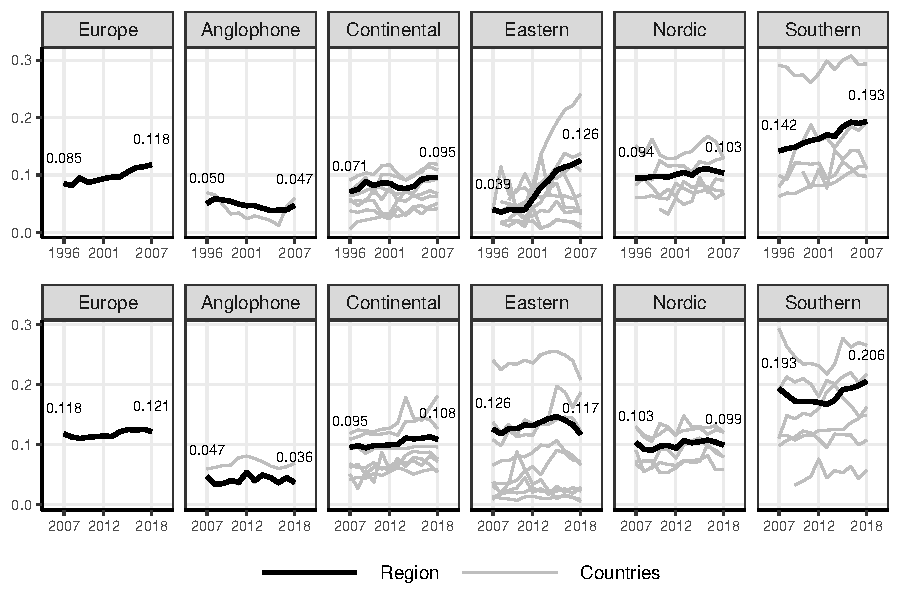
\includegraphics{../graphs/eu_lfs/graph_rate_region.pdf}}
    \label{graph_eu_lfs_rate_region}

    \footnotesize{Note: Authors calculations using LFS data.  Each cell shows the temporary employment rate for a given region, year, as shown by the thick, black line.  Country, region specifications are shown in table \ref{table_country_panel_years} in Appendix \ref{appendix_tables}.  Before 2007, levels are rising.  After 2007, levels are constant.  In the Eastern region, Poland stands out, with high and rising levels before 2007, but stagnating levels afterward.  In the Southern region, Spain stands out, with high, but declining levels, especially after 2007.  Italy and the Netherlands are among the few countries with high and rising levels before and after 2007.}
\end{figure}


\begin{sidewaysfigure}[htp!]
    \caption{Temporary employment rate over time, by demographic group (1996 - 2007)}
    \resizebox{\textwidth}{!}{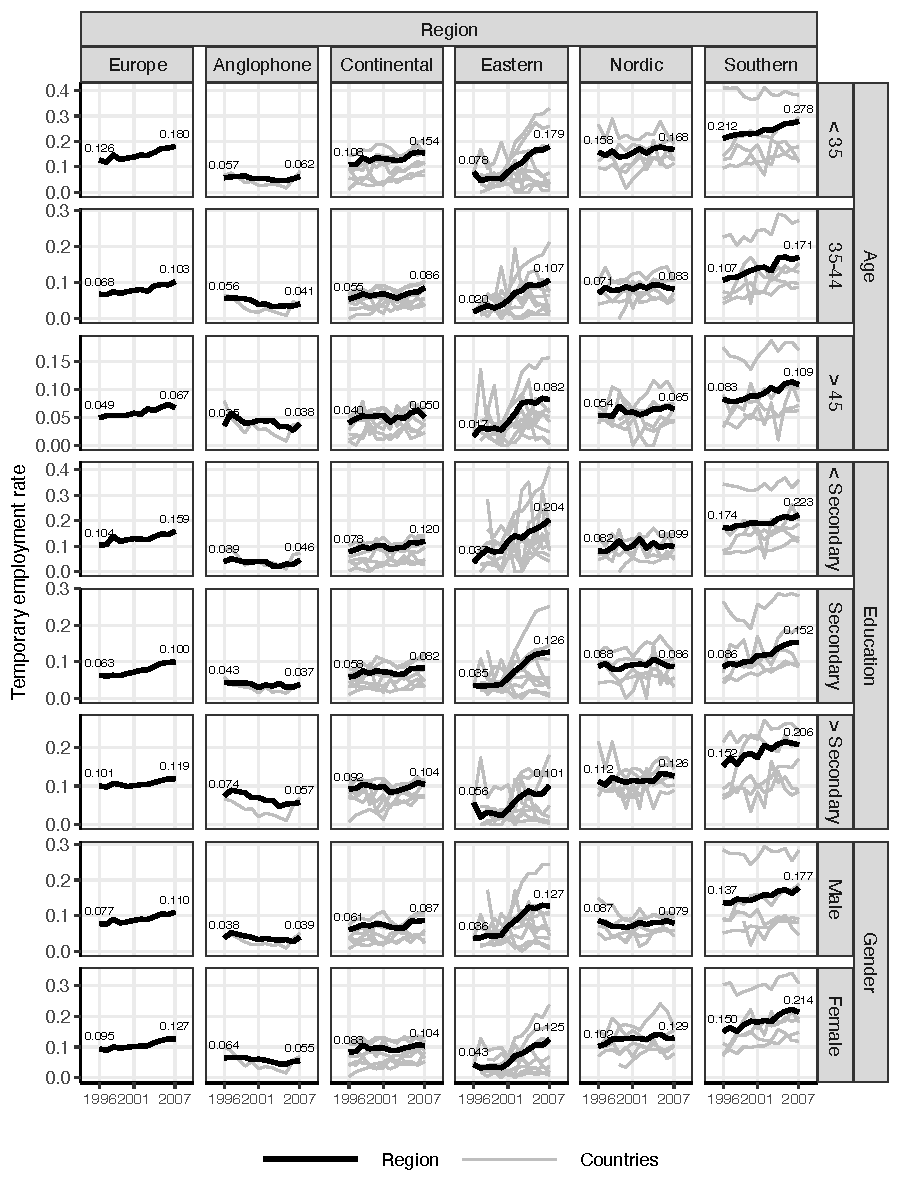
\includegraphics{../graphs/eu_lfs/graph_ftc_rate_region_country_group_period_1.pdf}}
    \label{graph_eu_lfs_pct_combo_1}
    \footnotesize{Note: Authors calculations using LFS data.  Each cell shows the temporary employment rate for a given region, year, demographic group.  For easier interpretation, highlighted subplots indicate where the temporary employment rate rose at least 1 percentage point and 10\% between 1996 and 2007.  Before 2007, the temporary employment rate is rising in almost every region and subgroup, except in the Anglophone and Nordic regions and among those with higher levels of education.}
\end{sidewaysfigure}

\begin{sidewaysfigure}[htp!]
    \caption{Temporary employment rate over time, by demographic group (2007 - 2019)}
    \resizebox{\textwidth}{!}{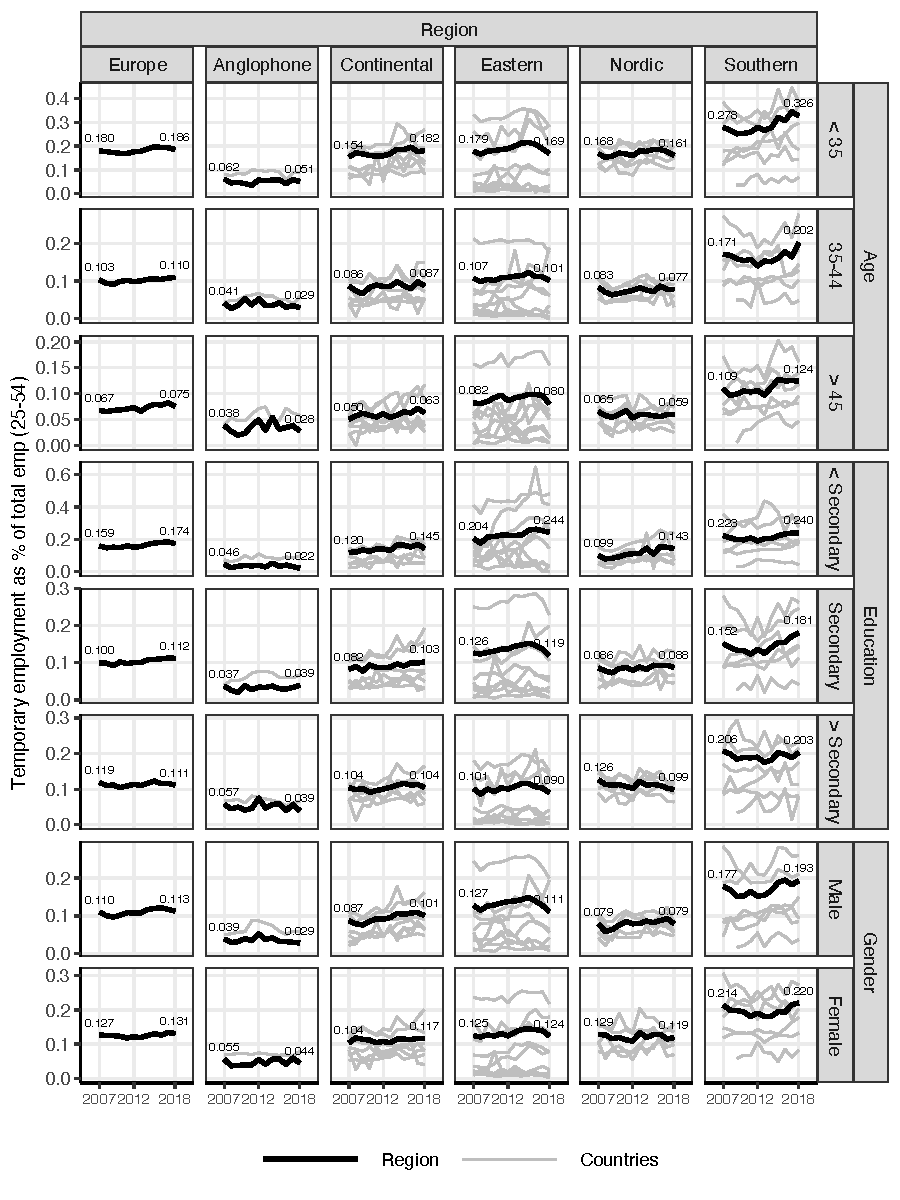
\includegraphics{../graphs/eu_lfs/graph_ftc_rate_region_country_group_period_2.pdf}}
    \label{graph_eu_lfs_pct_combo_2}    
    \footnotesize{Note: Authors calculations using LFS data.  Each cell shows the temporary employment rate for a given region, year, demographic group.  For easier interpretation, highlighted subplots indicate where the temporary employment rate rose at least 1 percentage points and 10\% between 2007 and 2019. After 2007, the temporary employment rate is constant within almost all demographic groups and regions.  However, there are two exceptions.  In the Southern region, the rate continues to rise in every demographic group, except those with higher levels of education.  Further, among those with lower levels of education, the rate continues to rise in every region, except the Anglophone region.}
\end{sidewaysfigure}

% Graphs - SILC

\clearpage
\begin{sidewaysfigure}[htp!]
    \caption{Predicted probability of a temporary contract}
    \resizebox{\textwidth}{!}{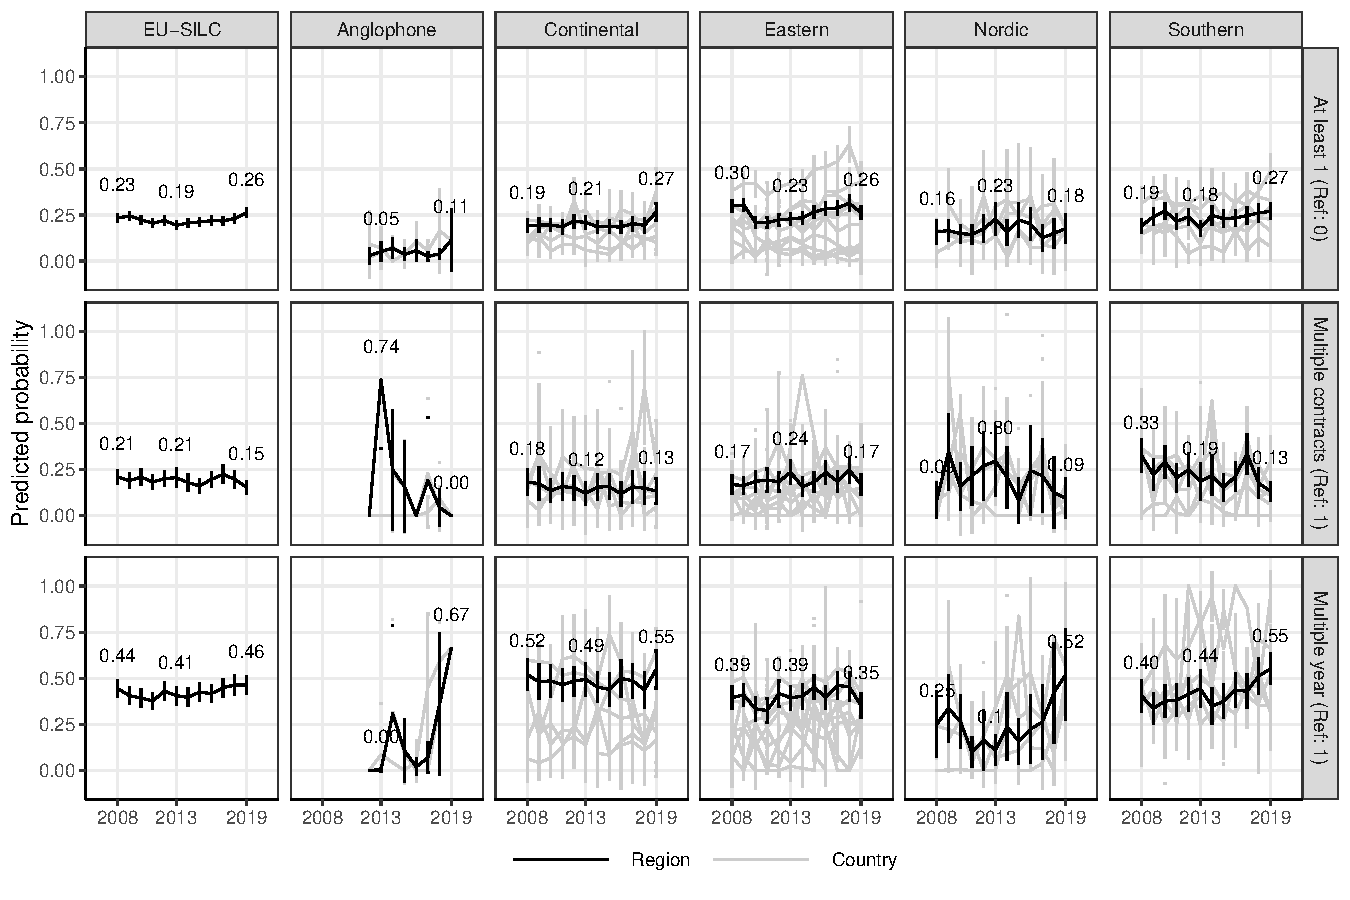
\includegraphics{../graphs/eu_silc/graph_eu_silc_glm_yhat_wt.pdf}}
    \label{graph_glm_yhat}
    \footnotesize{Note: Authors calculations using SILC data.  First row plots the probability of experiencing at least one temporary contract (ref: 0).  Second row plots the probability of experiencing multiple temporary contracts (ref: 1).  Third row plots the probability of experiencing a temporary contract that is multiple years long (ref: 1).  The interpretation is that temporary employment risk is rising, but the relative insecurity of temporary employment may be declining as the risk of receiving a multi-year contract is rising and the risk of receiving multiple contracts is constant or declining.}
\end{sidewaysfigure}

% Graphs - average marginal effect
\begin{sidewaysfigure}[htp!]
    \caption{AME of main effects on the probability of experiencing a temporary contract}
    \resizebox{\textwidth}{!}{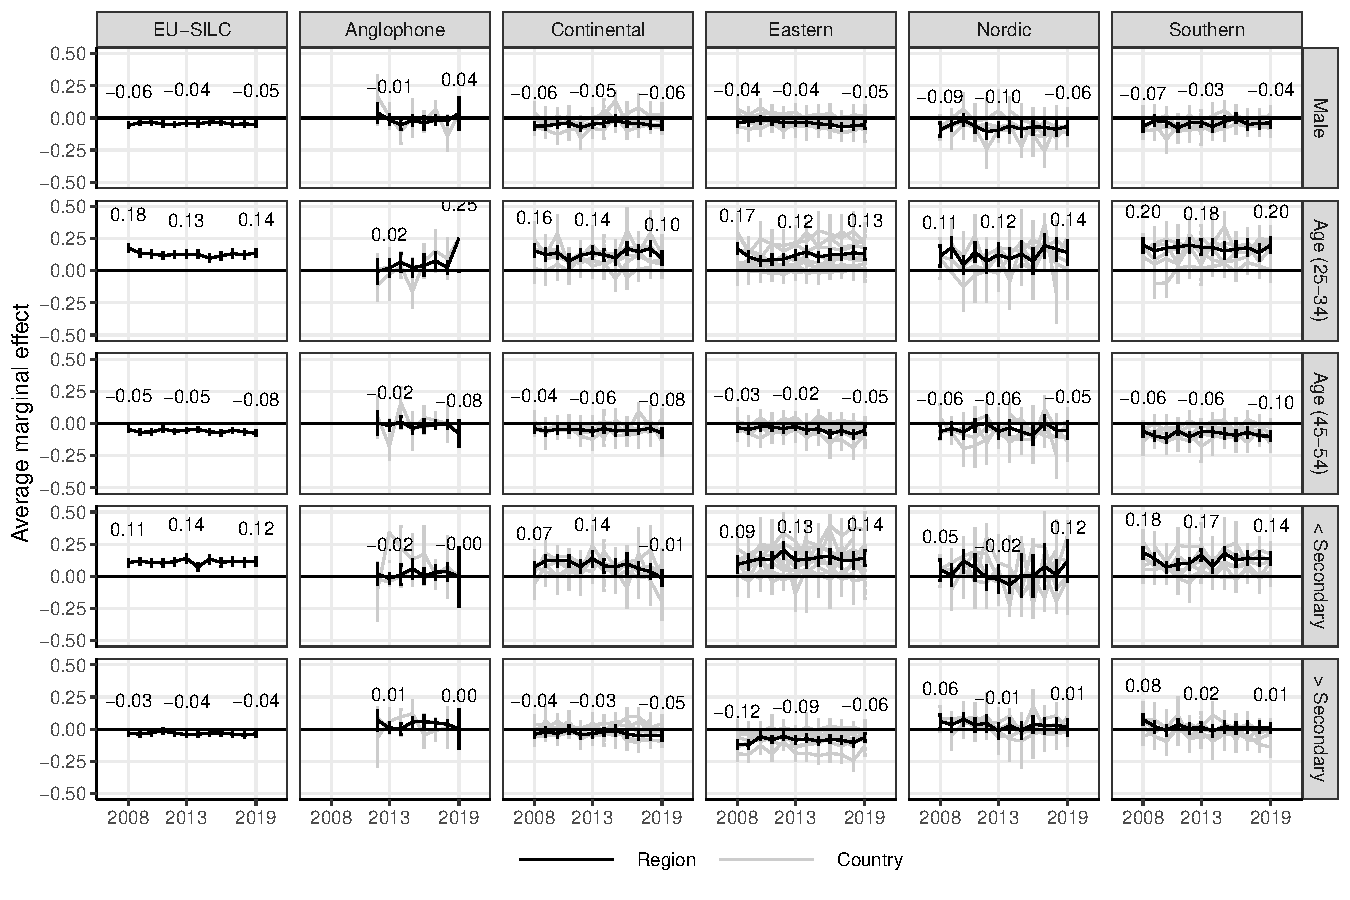
\includegraphics{../graphs/eu_silc/graph_eu_silc_glm_mfx_ever_wt.pdf}}
    \label{graph_glm_mfx_ever}
    \footnotesize{Note: Authors calculations using SILC data.  Plots the average marginal effect of independent variables on the probability of experiencing at least 1 temporary contract (ref: 0).  Between groups, risk is higher among women, younger workers, and those with lower levels of education.  However, within groups, there is little change in the demographic distribution of that rising risk.}
\end{sidewaysfigure}

\clearpage
\begin{sidewaysfigure}[htp!]
    \caption{AME of main effects on the number of temporary contracts}
    \resizebox{\textwidth}{!}{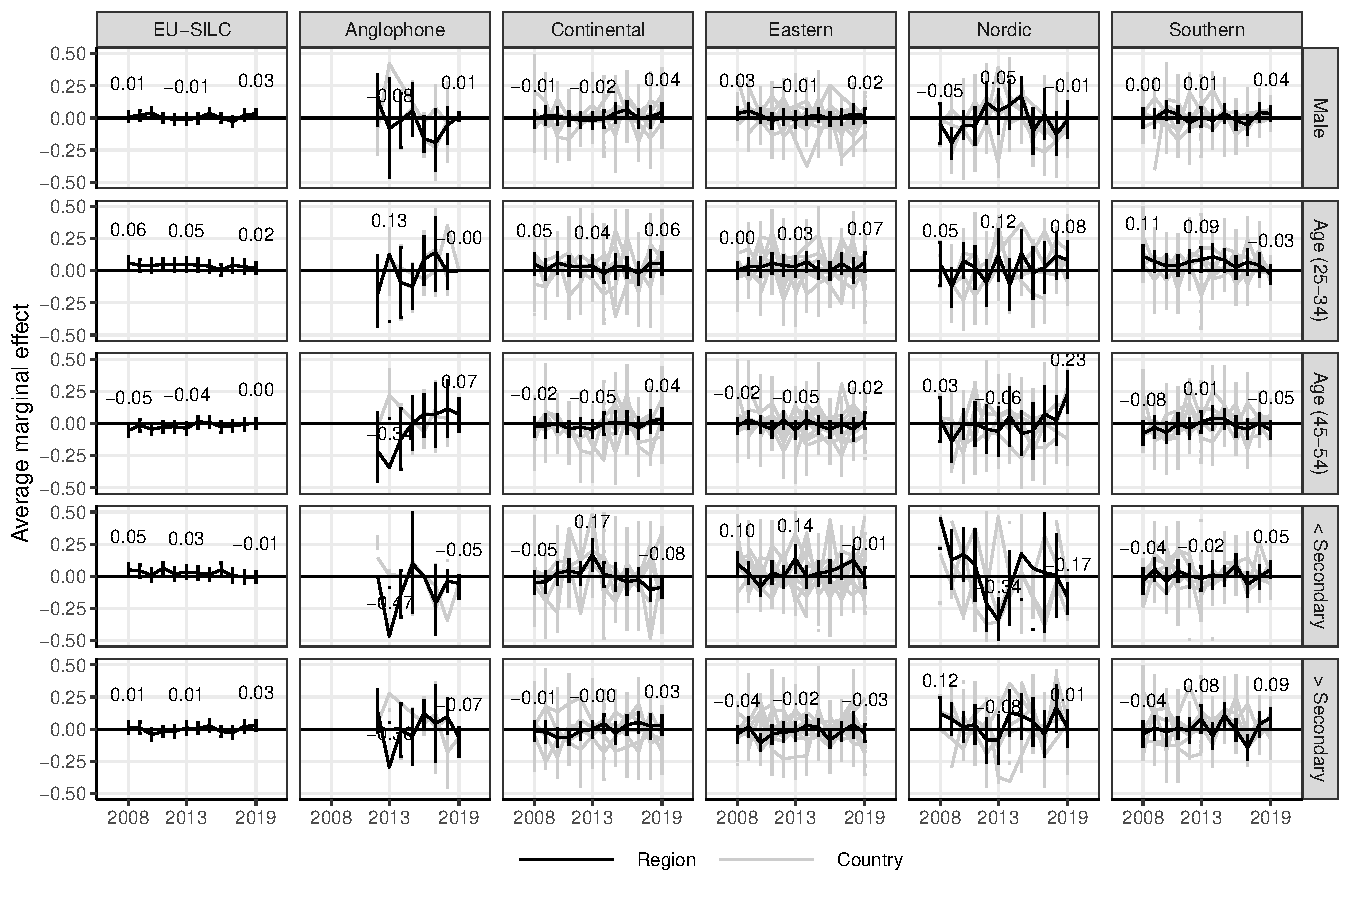
\includegraphics{../graphs/eu_silc/graph_eu_silc_glm_mfx_num_wt.pdf}}
    \label{graph_glm_mfx_num}
    \footnotesize{Note: Authors calculations using SILC data.  Plots the average marginal effect of independent variables on the probability of experiencing at least 2 temporary contracts (ref: 1).  In general, risk of multiple contracts is distributed equally between demographic groups.  Further, there is little change in the distribution of risk within demographic groups.}
\end{sidewaysfigure}

\clearpage
\begin{sidewaysfigure}[htp!]
    \caption{AME of main effects on the duration of temporary contracts}
    \resizebox{\textwidth}{!}{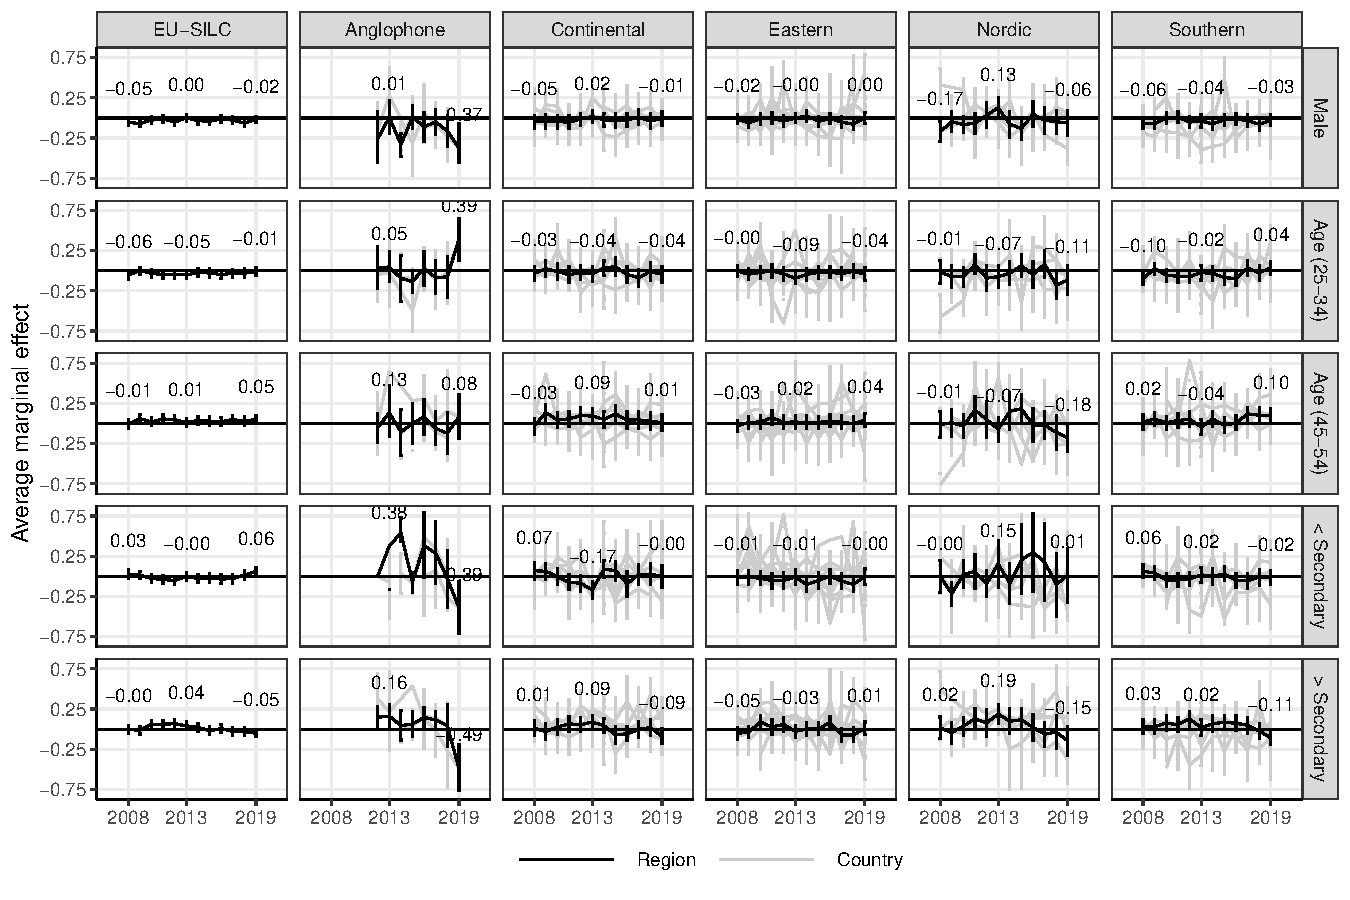
\includegraphics{../graphs/eu_silc/graph_eu_silc_glm_mfx_dur_wt.pdf}}
    \label{graph_glm_mfx_dur}
    \footnotesize{Note: Authors calculations using SILC data.  Plots the average marginal effect of independent variables on the probability of experiencing a temporary contract that is at least 2 years long (ref: 1). In general, risk of multi-year contracts is distributed equally between demographic groups.  Further, there is little change in the distribution of risk within demographic groups.}
\end{sidewaysfigure}

%%%%%%%%%%%%%%%%%%%%%%%%%%
%APPENDIX
%%%%%%%%%%%%%%%%%%%%%%%%%%

\clearpage
\appendix
\setcounter{table}{0}
\setcounter{figure}{0}
\renewcommand*\thetable{\Alph{section}.\arabic{table}}
\renewcommand*\thefigure{\Alph{section}.\arabic{figure}}
\renewcommand{\theHfigure}{\Alph{section}.\arabic{table}}
\renewcommand{\theHtable}{\Alph{section}.\arabic{figure}}

\section{Appendix: Sample selection}
\label{appendix_sample}

We apply the following sample selection criteria to the EU-SILC, as shown in table \ref{tables_steps_silc_4}.  There are three main filters.  First, we apply country, panel-level filters.  We restrict all panels to study windows that are four-years long.  While the majority of countries use a four-year long panel, a few use longer study windows.  We exclude country, panel waves with a temporary employment rate of zero or missing.  This affects three countries, Denmark, the United Kingdom, and Iceland.\footnote{Denmark in years between 2005 and 2010 (panel waves 2008 to 2013), the United Kingdom in 2008 (panel waves 2008 to 2011), and Iceland in 2009 (2009 panel waves).}  Furthermore, we exclude countries with less than 3 panel waves because 3 periods are necessary to create a trend.  This only affects Germany, which is only present in panel waves 2018 and 2019.

We use 12 panel waves, between 2008 and 2019.  2019 is the most recent year data is available.  Waves prior to the 2007 panel wave only include three years of observational data and the 2007 panel wave only includes 15 countries, compared to 25 or more countries in the other surveys.  Further, after all sample selection criteria are applied, there are only four countries in the 2007 panel wave, compared to 18 in the 2008 panel wave.  The result is 13.502.253 observations in 346 country, panel waves.  

Second, we apply individual-level filters.  The data includes individuals who are prime age (25-54), for the same reasons about the relationship between (in)voluntariness and age with respect to the LFS data, active labor market participants, and have a non zero personal weight.\footnote{There are two exceptions.  In the Netherlands, in panel waves 2016 -- 2019, the personal weight for all observations in the first year of a given panel wave is zero.  Similarly, in Norway, beginning with the 2010 panel waves, only last observation in panel period has personal weight greater than 0.  In these country, panel waves, we recode the personal base weight for these observations in these years as 1 and keep the observations, conditional on meeting all other criteria.}  We exclude individuals who were never employed in a four-year panel wave, otherwise there is no possibility of experiencing temporary employment.  We drop observations with missing values on education, gender, age, and contract type.  The result is 3.675.604 observations in 346 country, panel waves in the sample. 

Third and finally, we apply individual, panel-level filters.  The data only include individuals who are observable in each year of a given four-year panel wave.  Further, we exclude observations with missing or zero longitudinal panel weights, which weights for the inverse probability of being in the sample for the entire panel wave.  This leaves 1.058.840 total observations (264.710 unique observations) in 325 country, panel waves.  This is our `main' dataset.  We note that while not every country is in every panel wave, of the 31 countries in the sample, 23 countries are in at least nine panel waves, as shown in table \ref{table_country_panel_years}.  

To examine our three outcomes of interest, we create three sub datasets from the main dataset.  The first dependent variable is experiencing at least one temporary contract in a given four-year panel wave (i.e. ever).  The reference is an individual who does not experience a temporary contract (i.e. never).  To estimate this outcome, we aggregate the main dataset so each individual is present once in a given country, panel wave.  The result is dataset \emph{A} with 264.710 person, country, panel observations.  

Next, we determine temporary employment `spells' in order to estimate the probability of experiencing temporary employment, by the number and duration of temporary contracts.  We calculate temporary employment spells for each individual in a given country, panel wave using a variable in the dataset that asks, ``Change of job since last year?''  If an individual had a temporary contract in two consecutive time periods, but did not change jobs, then they had one temporary contract for two years.  By contrast, if an individual in two consecutive time periods had a temporary contract, but did change jobs, then they had two temporary contracts, each of which was one year.

The second dependent variable is experiencing two or more, i.e. multiple, temporary contracts in a given panel wave.  The reference is experiencing one, single temporary contract in that same panel wave.  To examine this outcome, we filter from dataset \emph{A} on the condition of ever experiencing temporary employment.  The result is dataset \emph{B} with 48.940 person, country, panel wave observations.  

The third dependent variable is experiencing a temporary contract that is two or more years long, i.e. multiple years.  The reference group is experiencing a temporary contract that is one, single year long.  To examine this outcome, we aggregate the main dataset so each spell of temporary employment is present once in a given country, panel wave, but an individual with multiple spells is present as many times as they have spells in a given country, panel wave.  Further, we filter on the condition of ever experiencing temporary employment.  The result is dataset \emph{C} with 59.582 person-spell, country, panel observations. 

We exclude variables related to income, occupation, and industry.  While including these additional variables into our analysis would improve model fit, it is not clear the degree to which these variables are related to the individual, job, or structural conditions.  For example, in Germany, occupational closure in the form of tasks and credentials are important determinants of temporary employment levels within a given occupation, ranging from 0 to 64 percent \citep{stuth_2017}.  We also do not control for individual self-selection into temporary employment.  Further, instead of relying on a single, unified, multi-level models, we use separate regression models for each panel wave in each country.  In so doing, we ensure that results are a reflection of the data, not model specification.

We use the methods and data describe above to quantify inequalities in temporary employment trends over time as well as between and within countries and demographic groups.  The goal is not to causally isolate an ``effect'' of country and demographic groups on temporary employment risk net of a large number of control variables, nor the consequences of temporary employment, as other research does.  Instead, the primary goal is descriptive.  Results provide a more accurate and representative accounting of levels and trends in temporary employment rate and risk than is otherwise reported, which helps to isolate the source of rising insecurity associated with temporary employment.  Replication files are made available by the authors on GitHub.

\subsection{Sensitivity}

Here, we address several important issues of sensitivity, which we divide into two main parts.  One main part is the sensitivity of the results within a given data set to our particular sample selection criteria.  With respect to the LFS, conditional on being a prime-age worker (25-54) and employed, the other selection criteria reduce the sample by 23.5\% (as shown in table \ref{tables_steps_lfs}).  Of these criteria, the most important one is a contract type, which accounts 17 percentage points.  While contract type is an essential variable required to determine temporary employment rate, results are not sensitive to the inclusion or exclusion of the other selection criteria.  

With respect to the SILC, the most important criteria is the requirement that observations be in the sample for all 4 years of a panel period.  This reduces the sample by 71\% (as shown in table \ref{tables_steps_silc_4}).  Alternatively, if we only require an individual to be in the first 2 years of a 4 year panel period, we only lose 37\% of all cases (as shown in table \ref{tables_steps_silc_2}).  While results are qualitatively similar, as shown in figure \ref{graph_eu_silc_compare_2_4_year_panel}, we use a longer time period owing to the application of a life course approach.  Further, results are qualitatively similar using unadjusted, non-parametric data, as shown in figure \ref{graph_eu_silc_compare_2_4_year_panel}.  

The second main part is issue of whether the results are sensitive to the choice of data set used.  Or, put another way, what is the degree to which the samples from the two data sets are comparable?  One way the samples are different is that the LFS sample only include those who are employed, which is how one calculates the temporary employment rate, while the SILC sample include all labour force participants, employed or unemployed.  We compare the temporary employment rate among the employed population to the rate among the employed and unemployed.  Trends are qualitatively similar, as shown in \ref{graph_rate_region_compare_lmp}.  

Another issue of comparison is that it is possible to use the SILC data in a cross-sectional form, as we described above, as well as the 4-year sample we use for our analysis, and the 2-year sample we use for sensitivity.  We compare the annual temporary employment rate between all three versions of SILC sample to LFS sample.  Results are qualitatively similar, as shown in figure \ref{graph_eu_silc_compare_SILC_LFS}.  


\clearpage
\section{Appendix: Tables}
\label{appendix_tables}

\begin{table}[h!]	
	\caption{Sample selection (EU-SILC, 4 year panel)}
    \resizebox{\textwidth}{!}{\begin{tabular}{l>{\raggedright\arraybackslash}p{1in}ll>{\raggedright\arraybackslash}p{4in}}
   \\[-1.8ex]\hline \\ 
 [-1.8ex]
\multicolumn{1}{l}{Step} & 
\multicolumn{1}{>{\raggedright\arraybackslash}p{1in}}{Country, panel periods} &
\multicolumn{1}{>{\raggedright\arraybackslash}p{1in}}{Unique observations} &
\multicolumn{1}{l}{\% $\Delta$} & 
\multicolumn{1}{l}{Notes} 
\\  

 \hline
0 & 377 & 5.961.876 &  & Raw data \\ 
  1 & 346 & 5.492.337 & -8\% & Country panel filters: Drop 2007 panel period.  Every panel period can only have four years.  Each country, panel, year must have non-missing temporary employment rate $>$ 0 \\ 
  2 & 346 & 2.278.772 & -59\% & Individual filters: prime age (25 - 54), active labor market participation (employed or unemployed), personal weight $>$ 0 \\ 
  3 & 346 & 2.082.421 & -9\% & Must be employed at least once \\ 
  4 & 346 & 1.588.269 & -24\% & Case-wise deletion of missing variables on education, gender, age, and contract type \\ 
  5 & 331 & 267.846 & -83\% & Individuals in each year of 4 year panel period \\ 
  6 & 325 & 264.710 & -1\% & Must have 4 year longitudinal weight (`Main dataset') \\ 
   \hline 
7 & Dataset \emph{A} & 264.710 &  & Main data:  One observation per individual, panel wave (ever) \\ 
  8 & Dataset \emph{B} & 48.940 &  & Dataset \emph{A}:$|>= 1$ temporary contract (number) \\ 
  9 & Dataset \emph{C} & 59.582 &  & Main data:$|>= 1$ temporary contract, one observation per spell, panel wave (duration) \\ 
   \hline 
 \hline 
\end{tabular}
}
    \label{tables_steps_silc_4}
\end{table}

\begin{sidewaystable}[h!]
    \caption{Number of observations per country, panel wave (EU-SILC, 4 year panel)}
    \footnotesize
    \resizebox{\textwidth}{!}{\begin{tabular}{lrrrrrrrrrrrrrr}
   \\[-1.8ex]\hline \\ 
 [-1.8ex] \multicolumn{1}{l}{Country} & \multicolumn{12}{l}{Four-year panel period ending} & \multicolumn{2}{l}{Total} \\ 

                    \cmidrule(r){1-1} \cmidrule(r){2-13} \cmidrule(r){14-15} 

            & 2008 & 2009 & 2010 & 2011 & 2012 & 2013 & 2014 & 2015 & 2016 & 2017 & 2018 & 2019 & Observations & Periods \\ 
 \hline
\\[-1.8ex]
  Anglophone countries: &  &  &  &  & 1.164 & 2.832 & 3.076 & 3.900 & 3.504 & 5.820 & 5.632 & 840 & 26.768 &   8 \\ 
  \hspace{5mm} Ireland &  &  &  &  & 600 & 640 & 648 & 528 & 1.188 & 2.104 & 1.100 & 840 & 7.648 &   8 \\ 
  \hspace{5mm} United Kingdom &  &  &  &  & 564 & 2.192 & 2.428 & 3.372 & 2.316 & 3.716 & 4.532 &  & 19.120 &   7 \\ 
  \multicolumn{14}{l}{\phantom{empty}} \\
  Continental countries: & 19.900 & 25.220 & 27.640 & 27.396 & 29.232 & 22.392 & 24.076 & 23.420 & 23.572 & 22.220 & 20.344 & 20.628 & 286.040 &  12 \\ 
  \hspace{5mm} Austria & 2.424 & 2.388 & 2.552 & 2.504 & 3.040 & 2.832 & 2.460 & 2.432 & 2.356 & 2.540 & 2.328 & 2.664 & 30.520 &  12 \\ 
  \hspace{5mm} Belgium & 2.856 & 2.676 & 2.868 & 2.284 & 2.336 & 2.516 & 2.264 & 2.252 & 2.732 & 2.296 & 2.388 & 3.856 & 31.324 &  12 \\ 
  \hspace{5mm} France & 11.260 & 11.376 & 12.160 & 12.776 & 13.520 & 12.432 & 12.020 & 11.828 & 11.664 & 10.504 & 9.732 & 9.224 & 138.496 &  12 \\ 
  \hspace{5mm} Luxembourg &  & 6.808 & 6.980 & 7.052 & 7.748 & 1.860 & 1.932 & 1.880 & 2.028 & 1.792 & 1.220 & 2.284 & 41.584 &  11 \\ 
  \hspace{5mm} Netherlands & 3.360 & 1.972 & 3.080 & 2.780 & 2.588 & 2.752 & 2.744 & 2.376 & 2.416 & 2.276 & 2.012 & 2.600 & 30.956 &  12 \\ 
  \hspace{5mm} Switzerland &  &  &  &  &  &  & 2.656 & 2.652 & 2.376 & 2.812 & 2.664 &  & 13.160 &   5 \\ 
  \multicolumn{14}{l}{\phantom{empty}} \\
  Eastern countries: & 27.604 & 32.044 & 34.020 & 32.632 & 34.352 & 36.128 & 36.900 & 33.148 & 38.328 & 35.040 & 38.200 & 37.260 & 415.656 &  12 \\ 
  \hspace{5mm} Bulgaria &  & 1.664 & 1.684 & 2.892 & 3.240 & 2.576 & 2.456 & 2.388 & 6.384 & 6.208 & 5.980 & 6.200 & 41.672 &  11 \\ 
  \hspace{5mm} Croatia &  &  &  &  &  & 2.048 & 1.908 & 1.824 & 1.728 & 2.284 & 3.704 & 3.504 & 17.000 &   7 \\ 
  \hspace{5mm} Czechia & 7.692 & 6.756 & 5.076 & 3.392 & 4.700 & 4.696 & 4.424 & 3.508 & 3.628 & 3.748 & 3.928 & 3.964 & 55.512 &  12 \\ 
  \hspace{5mm} Estonia & 1.004 & 2.940 & 2.808 & 2.596 & 2.176 & 2.532 & 2.316 & 2.796 & 2.672 & 2.652 & 2.264 & 2.856 & 29.612 &  12 \\ 
  \hspace{5mm} Hungary & 3.336 & 3.532 & 3.756 & 3.196 & 4.240 & 3.528 & 6.332 & 2.820 & 3.060 & 3.160 & 2.708 & 2.252 & 41.920 &  12 \\ 
  \hspace{5mm} Latvia & 1.684 & 1.828 & 2.044 & 2.564 & 2.436 & 2.556 & 2.424 & 2.168 & 2.024 & 1.832 & 2.052 & 1.912 & 25.524 &  12 \\ 
  \hspace{5mm} Lithuania & 1.884 & 2.712 & 2.744 & 2.520 & 2.472 & 2.892 & 2.132 & 2.340 & 1.760 & 2.424 & 1.596 & 1.900 & 27.376 &  12 \\ 
  \hspace{5mm} Poland & 6.556 & 6.812 & 6.196 & 5.408 & 5.488 & 5.924 & 5.696 & 5.972 & 5.148 & 4.988 & 3.980 & 3.956 & 66.124 &  12 \\ 
  \hspace{5mm} Romania &  &  & 3.516 & 3.512 & 3.300 & 3.484 & 3.108 & 3.276 & 3.376 & 3.320 & 3.708 & 3.428 & 34.028 &  10 \\ 
  \hspace{5mm} Serbia &  &  &  &  &  &  &  &  & 2.648 & 2.456 & 2.660 & 2.604 & 10.368 &   4 \\ 
  \hspace{5mm} Slovakia & 3.440 & 3.660 & 4.064 & 4.024 & 3.988 & 3.684 & 3.888 & 3.728 & 3.892 &  & 3.652 &  & 38.020 &  10 \\ 
  \hspace{5mm} Slovenia & 2.008 & 2.140 & 2.132 & 2.528 & 2.312 & 2.208 & 2.216 & 2.328 & 2.008 & 1.968 & 1.968 & 4.684 & 28.500 &  12 \\ 
  \multicolumn{14}{l}{\phantom{empty}} \\
  Nordic countries: & 4.560 & 6.872 & 7.576 & 6.604 & 6.108 & 6.180 & 6.588 & 5.868 & 6.148 & 5.660 & 5.612 & 5.148 & 72.924 &  12 \\ 
  \hspace{5mm} Denmark &  &  &  &  &  &  & 808 & 1.192 & 1.148 & 976 & 764 & 880 & 5.768 &   6 \\ 
  \hspace{5mm} Finland &  & 1.372 & 1.388 & 1.320 & 1.064 & 2.020 & 2.104 & 1.944 & 2.040 & 1.924 & 1.948 & 1.864 & 18.988 &  11 \\ 
  \hspace{5mm} Iceland & 608 &  & 568 & 672 & 636 & 556 & 552 & 532 & 532 & 480 & 440 &  & 5.576 &  10 \\ 
  \hspace{5mm} Norway & 3.952 & 3.728 & 3.484 & 3.140 & 2.896 & 2.192 & 2.004 & 1.304 & 1.340 & 1.220 & 1.252 & 1.344 & 27.856 &  12 \\ 
  \hspace{5mm} Sweden &  & 1.772 & 2.136 & 1.472 & 1.512 & 1.412 & 1.120 & 896 & 1.088 & 1.060 & 1.208 & 1.060 & 14.736 &  11 \\ 
  \multicolumn{14}{l}{\phantom{empty}} \\
  Southern countries: & 16.904 & 20.744 & 21.588 & 20.104 & 18.988 & 19.444 & 18.960 & 20.780 & 21.396 & 21.796 & 28.204 & 28.544 & 257.452 &  12 \\ 
  \hspace{5mm} Cyprus & 2.160 & 2.124 & 1.928 & 1.712 & 1.768 & 3.520 & 2.376 & 3.384 & 1.996 & 2.532 & 2.348 & 2.472 & 28.320 &  12 \\ 
  \hspace{5mm} Greece &  & 2.248 & 1.764 & 2.188 & 1.764 & 1.376 & 1.072 & 1.264 & 2.596 & 2.832 & 6.980 & 5.264 & 29.348 &  11 \\ 
  \hspace{5mm} Italy & 7.316 & 6.996 & 7.700 & 6.736 & 5.648 & 4.904 & 6.144 & 6.136 & 6.132 & 6.012 & 4.468 & 7.744 & 75.936 &  12 \\ 
  \hspace{5mm} Malta &  & 1.292 & 1.200 & 1.096 & 1.100 & 1.632 & 1.964 & 1.696 & 2.080 & 1.804 & 1.828 & 1.692 & 17.384 &  11 \\ 
  \hspace{5mm} Portugal & 1.868 & 1.964 & 2.252 & 1.860 & 2.624 & 2.624 & 2.940 & 3.248 & 3.576 & 3.520 & 7.280 & 6.792 & 40.548 &  12 \\ 
  \hspace{5mm} Spain & 5.560 & 6.120 & 6.744 & 6.512 & 6.084 & 5.388 & 4.464 & 5.052 & 5.016 & 5.096 & 5.300 & 4.580 & 65.916 &  12 \\ 
  \multicolumn{14}{l}{\phantom{empty}} \\
  EU-SILC & 68.968 & 84.880 & 90.824 & 86.736 & 89.844 & 86.976 & 89.600 & 87.116 & 92.948 & 90.536 & 97.992 & 92.420 & 1.058.840 & 325 \\ 
   \hline\hline \\[-1.8ex] 
\end{tabular}
}
    \label{table_country_panel_years}
\end{sidewaystable}

\begin{table}[h!]   
    \caption{Sample selection (EU-LFS)}
    \resizebox{\textwidth}{!}{\begin{tabular}{l>{\raggedright\arraybackslash}p{1in}ll>{\raggedright\arraybackslash}p{4in}}
   \\[-1.8ex]\hline \\ 
 [-1.8ex]
\multicolumn{1}{l}{Step} & 
\multicolumn{1}{>{\raggedright\arraybackslash}p{1in}}{Country, year periods} &
\multicolumn{1}{l}{Observations} & 
\multicolumn{1}{l}{\% $\Delta$} & 
\multicolumn{1}{l}{Notes} 
\\  

 \hline
0 & 708 & 85.678.076 &  & Raw data \\ 
  1 & 708 & 27.105.901 & -68\% & Year $>=$ 1996, employed, prime age (25 - 54) \\ 
  2 & 706 & 22.582.555 & -17\% & Observable contract type \\ 
  3 & 698 & 22.247.241 & -1\% & Observable education \\ 
  4 & 698 & 20.768.195 & -7\% & Personal weight $>$ 0 \\ 
   \hline 
\end{tabular}
}
    \label{tables_steps_lfs}
\end{table}

\begin{table}[h!]	
	\caption{Sample selection (EU-SILC, 2 year panel), as comparable to table \ref{tables_steps_silc_4}}
    \resizebox{\textwidth}{!}{\begin{tabular}{l>{\raggedright\arraybackslash}p{1in}ll>{\raggedright\arraybackslash}p{4in}}
   \\[-1.8ex]\hline \\ 
 [-1.8ex]
\multicolumn{1}{l}{Step} & 
\multicolumn{1}{>{\raggedright\arraybackslash}p{1in}}{Country-panel periods} &
\multicolumn{1}{l}{Observations} & 
\multicolumn{1}{l}{\% $\Delta$} & 
\multicolumn{1}{l}{Notes} 
\\  

 \hline
0 & 377 & 14.724.687 &  & Raw data \\ 
  1 & 346 & 13.502.253 & -8\% & Country panel filters: Drop 2007 panel period.  Every panel period can only have four years.  Each country, panel, year must have non-missing temporary employment rate $>$ 0 \\ 
  2 & 346 & 5.234.565 & -61\% & Individual filters: prime age (25 - 54), active labor market participation (employed or unemployed), personal weight $>$ 0 \\ 
  3 & 346 & 4.887.435 & -7\% & Must be employed at least once \\ 
  4 & 346 & 3.675.604 & -25\% & Case-wise deletion of missing variables on education, gender, age, and contract type \\ 
  5 & 345 & 2.307.656 & -37\% & Individuals in first 2 years of 4 year panel period \\ 
  6 & 343 & 1.914.466 & -17\% & Must have 2 year longitudinal weight (`Main dataset') \\ 
   \hline 
7 & Dataset \emph{A} & 957.233 &  & Main data:  One observation per individual, panel wave (ever) \\ 
  8 & Dataset \emph{B} & 151.015 &  & Dataset \emph{A}:$|>= 1$ temporary contract (number) \\ 
  9 & Dataset \emph{C} & 162.716 &  & Main data:$|>= 1$ temporary contract, one observation per spell, panel wave (duration) \\ 
   \hline 
 \hline 
\end{tabular}
}
    \label{tables_steps_silc_2}
\end{table}

\clearpage
\section{Appendix: Figures}
\label{appendix_figures}

\begin{sidewaysfigure}[htp!]
    \caption{Replicate figure \ref{graph_glm_yhat} with different EU-SILC samples}
    \resizebox{\textwidth}{!}{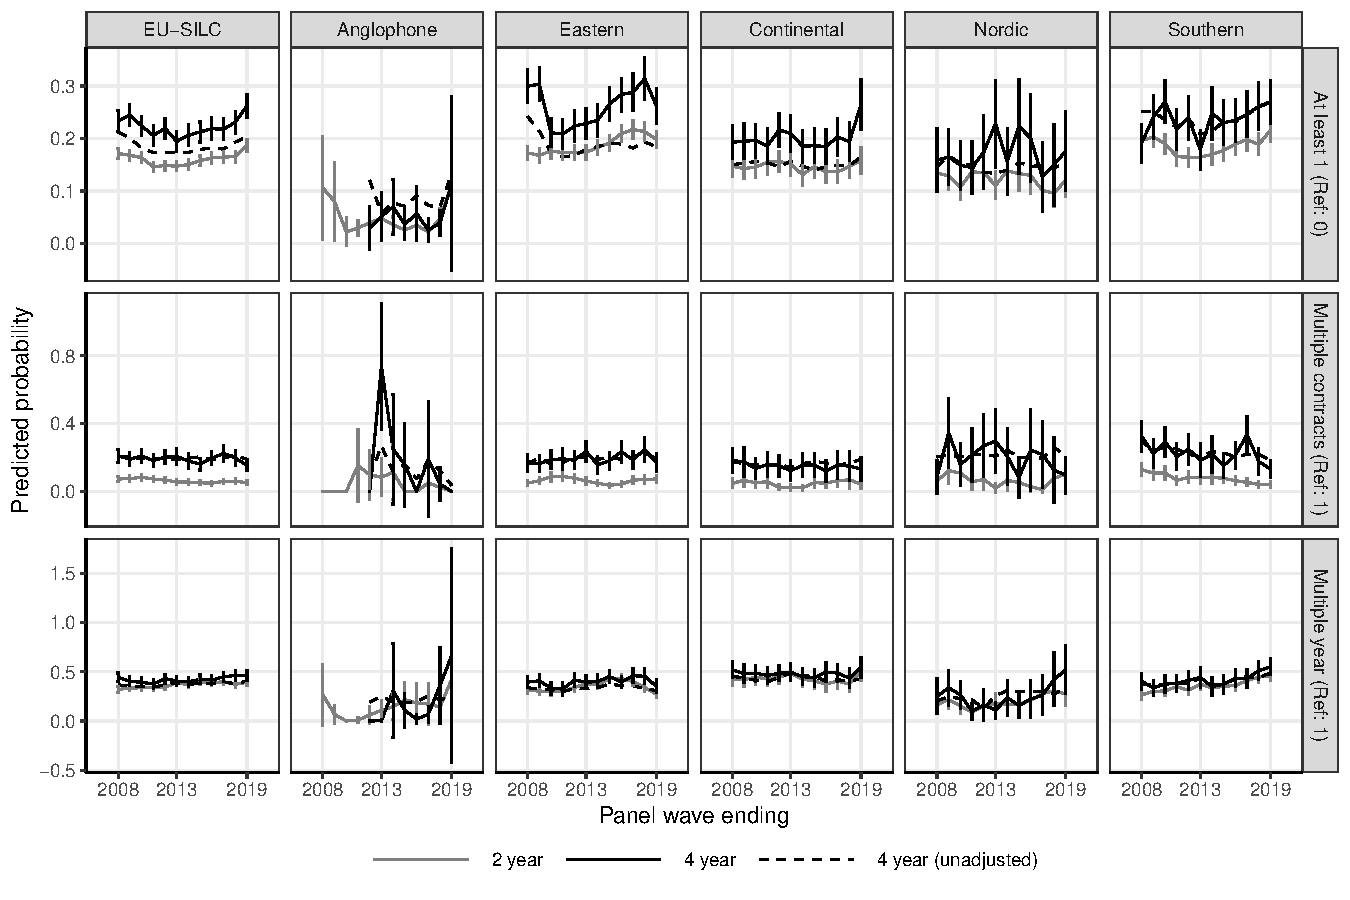
\includegraphics{../graphs/eu_silc/sensitivity/graph_eu_silc_compare_2_4_year_panel.pdf}}
    \label{graph_eu_silc_compare_2_4_year_panel}
    \footnotesize{Note: Authors calculations using SILC data.  The black, solid line is used in the main paper.  The gray, solid line applies the same sample selection strategy and applies the same model, but using a 2-year sample.  The black, dotted line uses the same sample selection strategy as the paper, but is not model adjusted.  Results are qualitatively similar.  The interpretation is that results are not a reflection of bias from model specification or sample attrition.}
\end{sidewaysfigure}

\begin{figure}[htp!]
    \caption{Replicate figure \ref{graph_eu_lfs_rate_region}, with different definitions of temporary employment rate}
    \resizebox{\textwidth}{!}{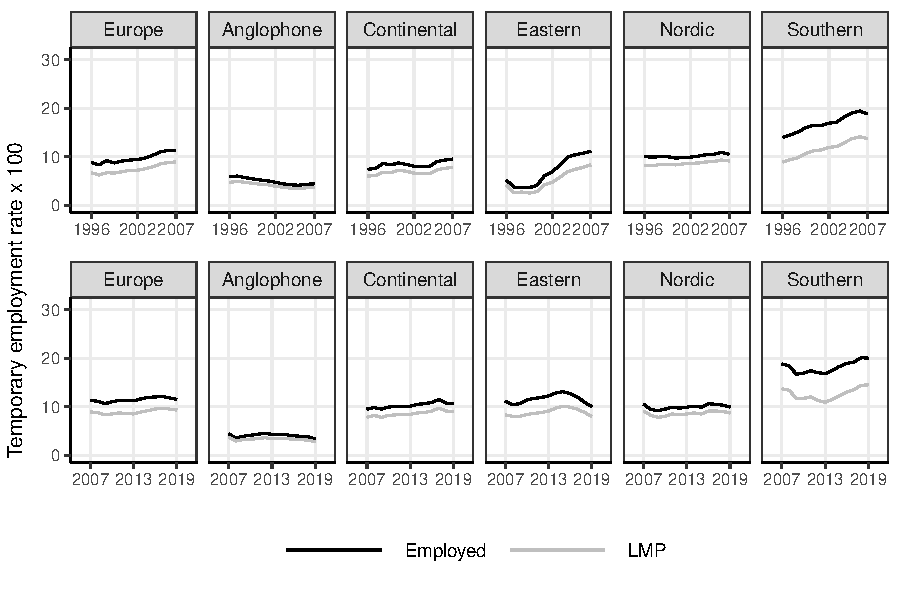
\includegraphics{../graphs/eu_lfs/sensitivity/graph_rate_region_compare_lmp.pdf}}
    \label{graph_rate_region_compare_lmp}
    \footnotesize{Note: Authors calculations using LFS data.  Each cell shows the temporary employment rate for a given region, year.  Black line shows the temporary employment rate among those who are employed in the LFS.  This is the standard way to calculate the temporary employment rate.  Gray line shows the temporary employment rate among those who are employed or unemployed in the LFS, i.e. labour market participants (LMP).  This is similar to the SILC sample.  The two lines are similar, although the rate is always lower using the sample of LMP, as we would expect.  The interpretation is that the temporary employment rate in the LFS is not driven by the sample selection strategy.}
\end{figure}

\begin{sidewaysfigure}[htp!]
    \caption{Comparing temporary employment rate across different data sources}
    \resizebox{\textwidth}{!}{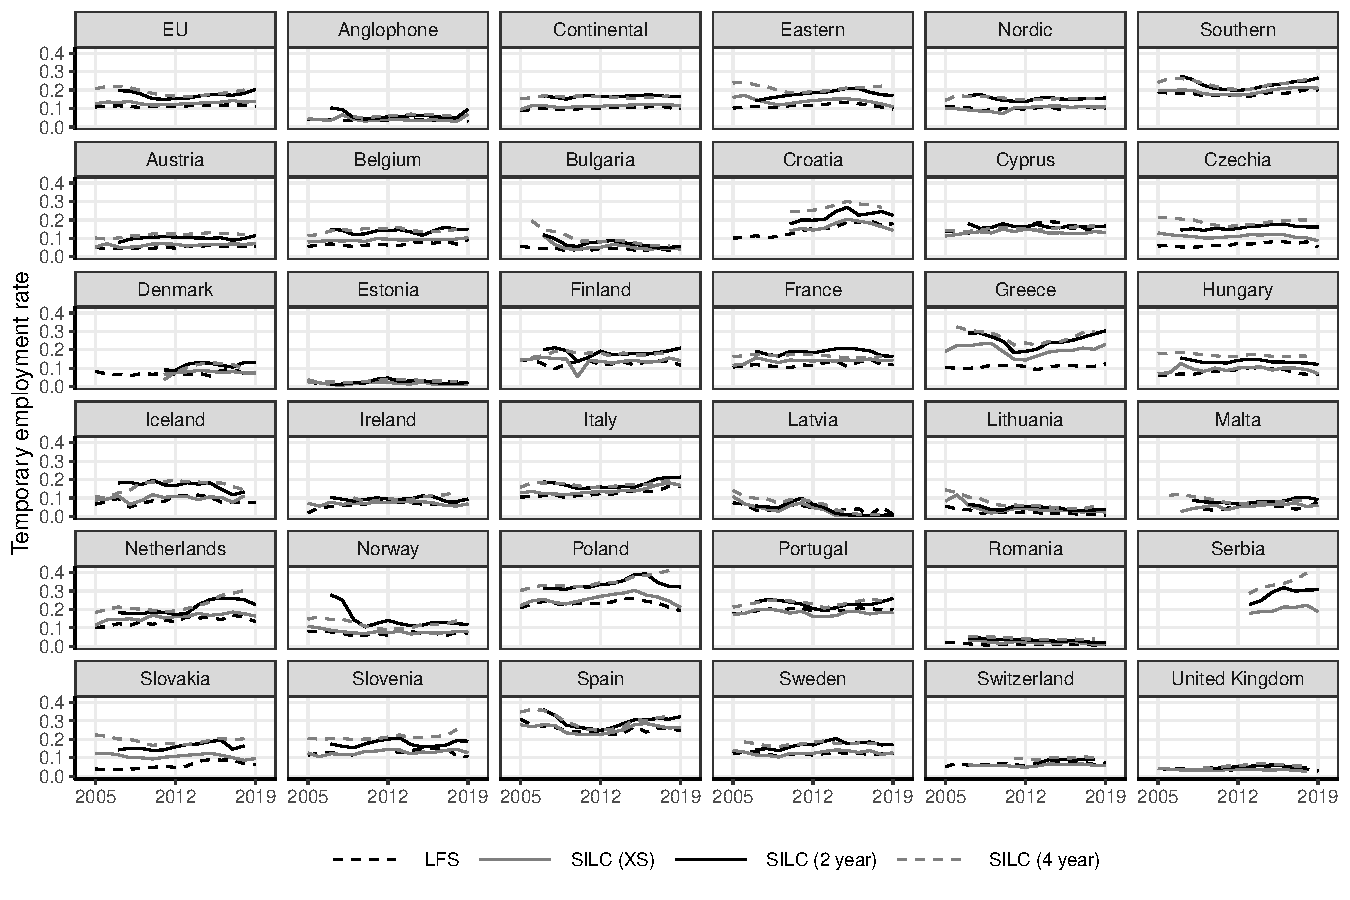
\includegraphics{../graphs/eu_silc/sensitivity/graph_eu_silc_compare_SILC_LFS.pdf}}
    \label{graph_eu_silc_compare_SILC_LFS}
    \footnotesize{Note: Authors calculations using LFS/SILC data.  Black, dotted line is temporary employment rate from cross-sectional, LFS data.  Gray, solid line is temporary employment rate from cross-sectional, SILC data.  Black, solid line is temporary employment rate from 2-year SILC sample.  Black, dashed line is temporary employment rate from 4-year SILC sample.  Temporary employment rate is similar, regardless of data type}
\end{sidewaysfigure}

\begin{figure}[htp!]
    \caption{Predicted probability of at least 1 temporary contract, by country}
    \resizebox{\textwidth}{!}{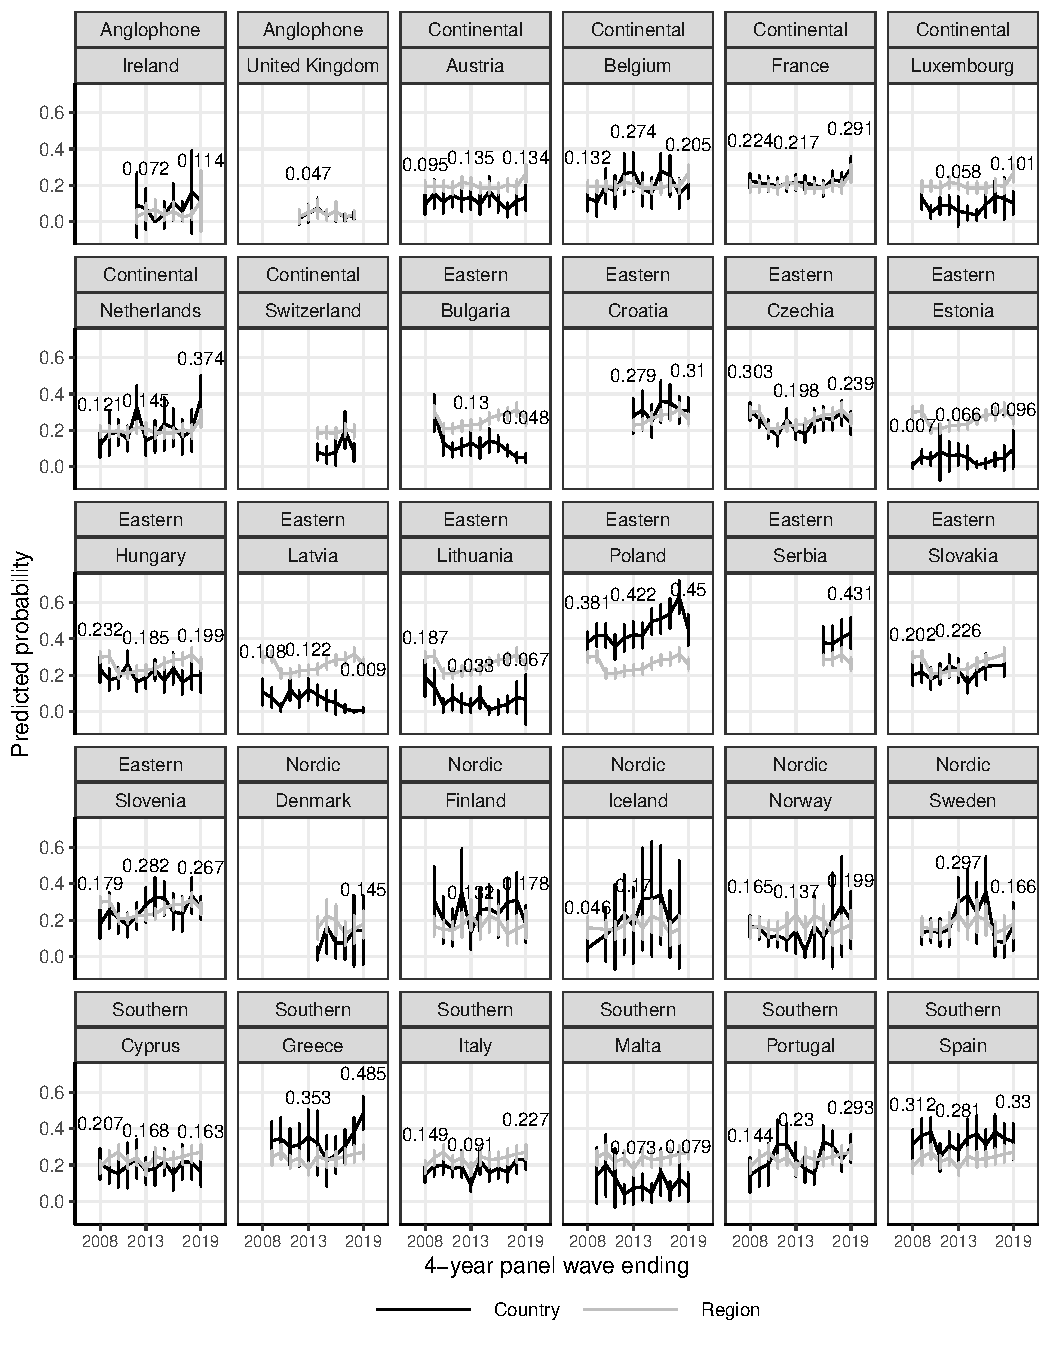
\includegraphics{../graphs/eu_silc/graph_eu_silc_glm_yhat_ever_country.pdf}}
    \label{graph_eu_silc_glm_yhat_ever_country}
    \footnotesize{Note: Authors calculations using SILC data.  Plots the probability of experiencing at least one temporary contract (ref: 0) from row 1 in figure \ref{graph_glm_yhat}, but with more country-level detail.  Each subplot is its own country.  Gray line is region-level.  Black line is country-level.}
\end{figure}

\begin{figure}[htp!]
    \caption{Predicted probability of a temporary contract (number), by country}
    \resizebox{\textwidth}{!}{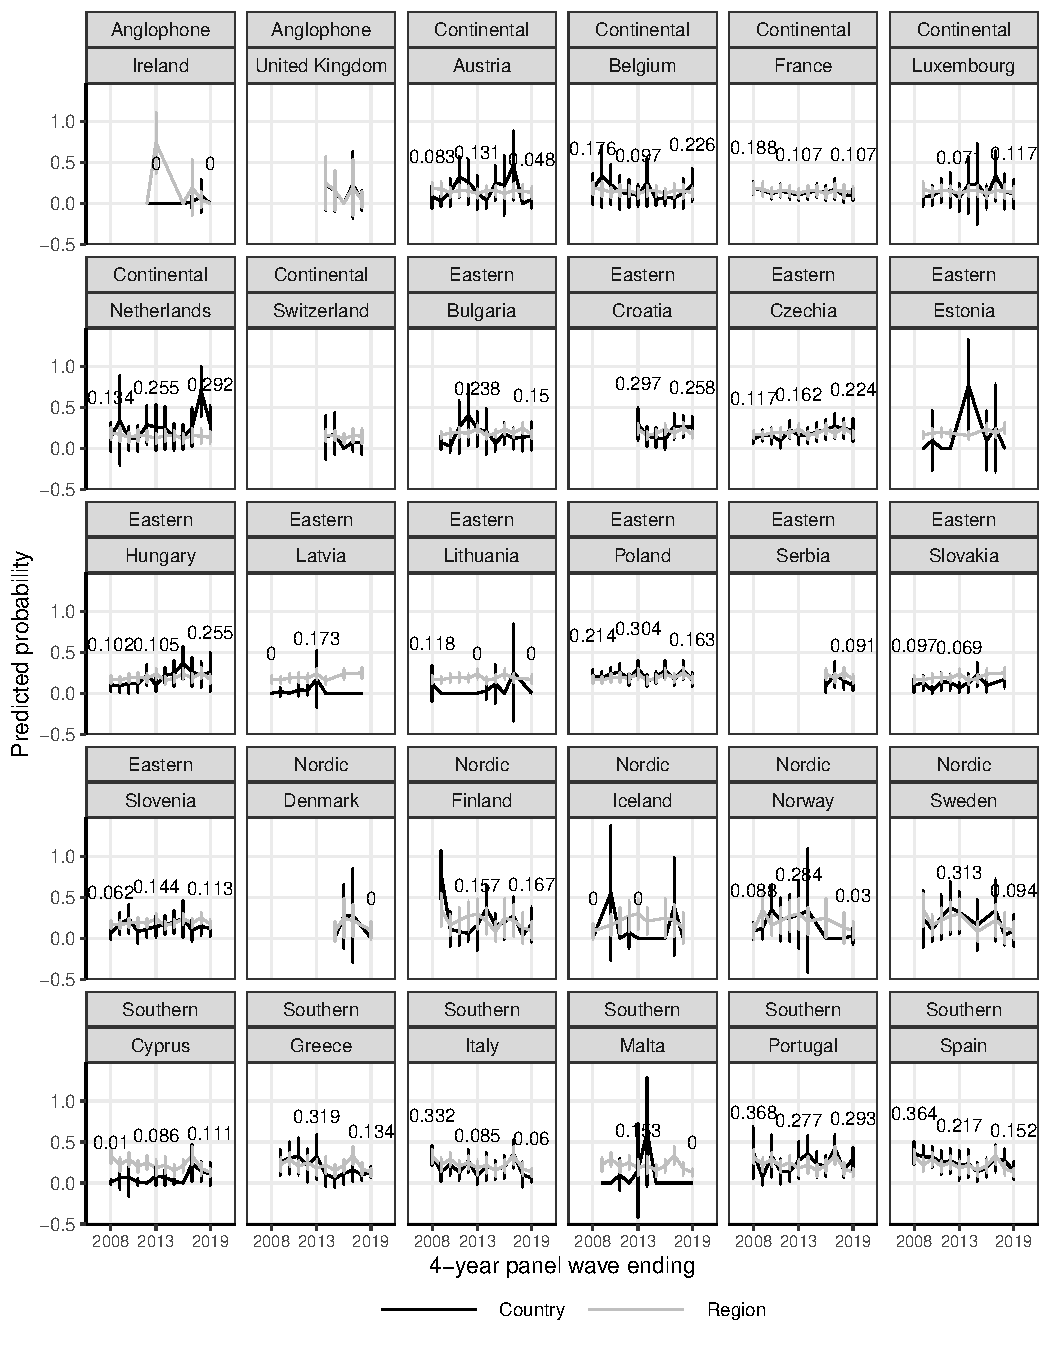
\includegraphics{../graphs/eu_silc/graph_eu_silc_glm_yhat_num_country.pdf}}
    \label{graph_eu_silc_glm_yhat_num_country}
    \footnotesize{Note: Authors calculations using SILC data.  Plots the probability of experiencing multiple temporary contracts (ref: 1) from row 2 in figure \ref{graph_glm_yhat}, but with more country-level detail.  Each subplot is its own country.  Gray line is region-level.  Black line is country-level.}
\end{figure}

\begin{figure}[htp!]
    \caption{Predicted probability of a temporary contract (duration), by country}
    \resizebox{\textwidth}{!}{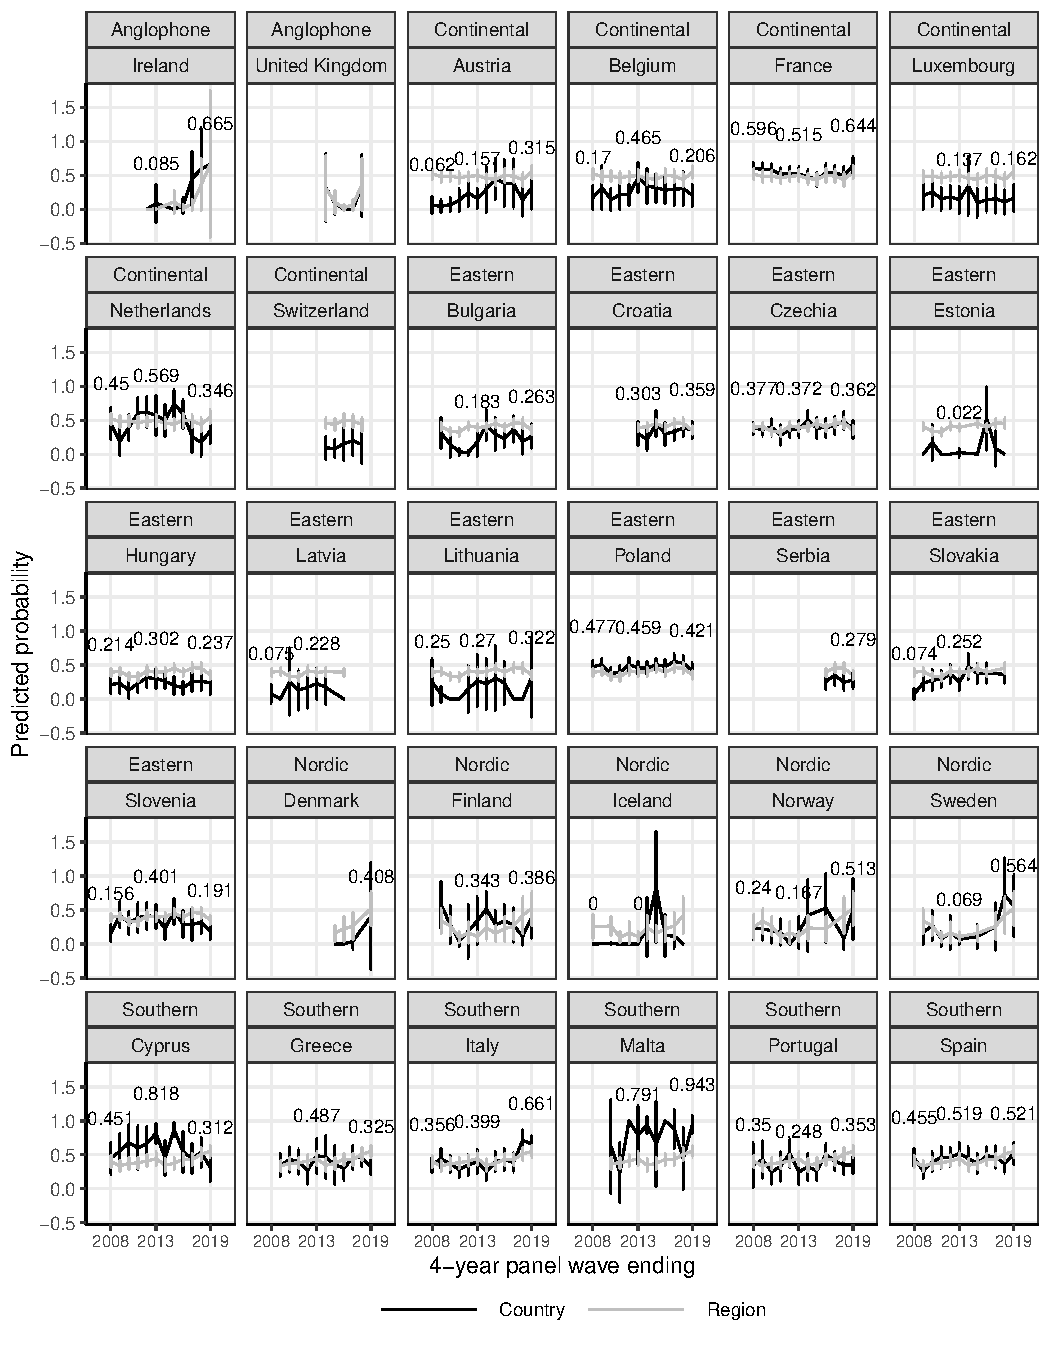
\includegraphics{../graphs/eu_silc/graph_eu_silc_glm_yhat_dur_country.pdf}}
    \label{graph_eu_silc_glm_yhat_dur_country}
    \footnotesize{Note: Authors calculations using SILC data.  Plots the probability of experiencing a temporary contract that is multiple years long (ref: 1) from row 3 in figure \ref{graph_glm_yhat}, but with more country-level detail.  Each subplot is its own country.  Gray line is region-level.  Black line is country-level.}
\end{figure}



\end{document}

